%% USPSC-Cap3-Conclusao.tex
% ---
% Conclusão
% ---
\chapter{Resultados}

Como resultados parciais foi possível observar os dados de mortes em geral, foi observado que as a mortalidade dos homens está em 54\% (\autoref{fig_dist_sexo}), apontando um possível desbalanceamento a ser investigas, além disto há uma incidência de motes de pessoas brancas de 73\% (\autoref{fig_dist_racacor}), este é um número a ser considerado com cautela, dado a problemática envolvendo o preenchimento dos dados apontado por \citeonline{muzy2021analise}.

\begin{figure}[H]
	\caption{\label{fig_dist_sexo}Distribuição do Sexo na amostra}
	\begin{center}
		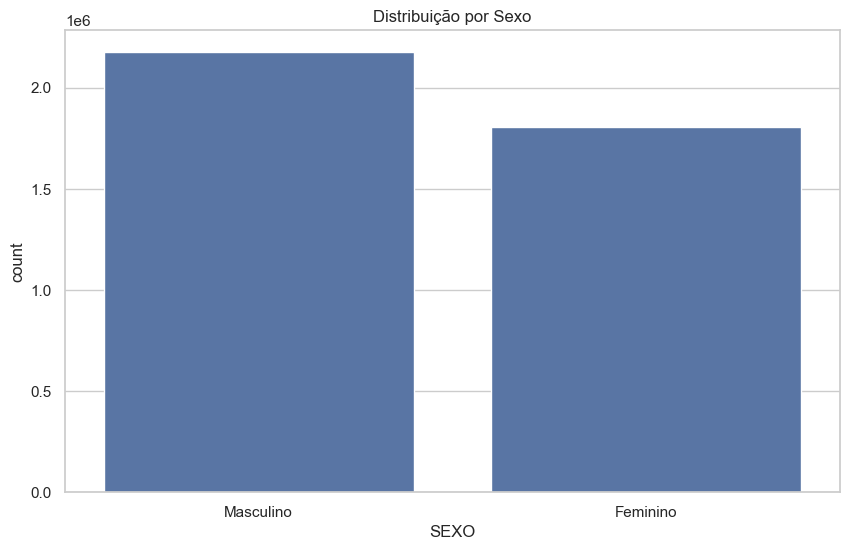
\includegraphics[width=.6\textwidth]{USPSC-img/dist-sexo.png}
	\end{center}
\legend{Fonte: SIM-DO e Resultados da Pesquisa}
\end{figure}

\begin{figure}[H]
	\caption{\label{fig_dist_racacor}Distribuição de Raça/Cor na amostra}
	\begin{center}
		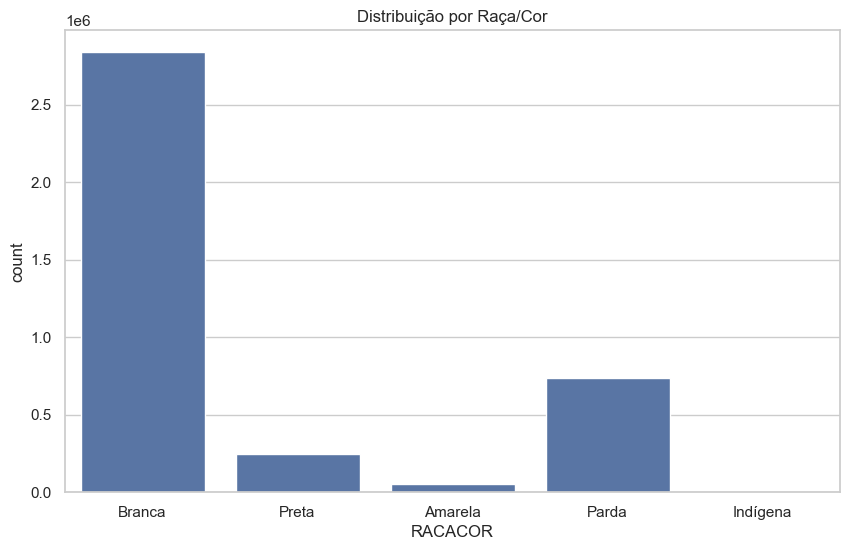
\includegraphics[width=.6\textwidth]{USPSC-img/dist_racacor.png}
	\end{center}
	\legend{Fonte: SIM-DO e Resultados da Pesquisa}
\end{figure}

Para a conclusão do trabalho é necessária a construção do \textit{Dashboard}, além de considerar as causas de morte de interesse inicial, no momento de conclusão deste relatório parcial está sendo utilizada a lista de causas evitáveis de morte proposta por \citeonline{malta2007lista}.

